\documentclass[10pt]{article}


%\usepackage{fullpage,epsfig,wrapfig,url,palatino,color}
\usepackage{epsfig,wrapfig,url,palatino,color}

\pagestyle{plain}

\renewcommand{\baselinestretch}{1.}

\setlength{\topmargin}{0in}
\setlength{\evensidemargin}{0in}
\setlength{\oddsidemargin}{0in}
\setlength{\headheight}{0in}
\setlength{\headsep}{0in}
\setlength{\footskip}{0.2in}
\setlength{\textheight}{9in}
\setlength{\textwidth}{6.5in}

\renewcommand{\topfraction}{0.99}
\renewcommand{\bottomfraction}{0.99}
\renewcommand{\textfraction}{0.01}
\renewcommand{\floatpagefraction}{0.01}
\renewcommand{\dbltopfraction}{0.99}
\renewcommand{\dblfloatpagefraction}{0.01}

\begin{document}

\noindent
{\bf Title of Proposal:}  Evaluation of the Virtual Heliodon for Architectural Daylighting Design\\
{\bf Researcher:}   Barbara Cutler\\
{\bf Address:}  MRC 331A\\
{\bf Phone:} 518 276 3274\\
{\bf Research Advisor (for students):}  N/A \\
{\bf Department:}  Computer Science \\
{\bf Is this proposal related to a sponsored project?}  Yes \\
{\bf If yes,  please indicate:}  \\
Existing Award: (Fund \# A12016), NSF, \\
Immersive Architectural Daylighting Design Experience \\

\noindent
All investigators, including faculty supervisors, on this project must
complete the self-study course on protection of human research
subjects. \\
{\bf Certification:  I/We have completed the course:} \\
Barbara M Cutler 7/2/08, refresher 11/2/11 \\
Joshua Nasman (CS PhD student) 10/21/09, refresher 4/1/13

\paragraph{Objective:}
%
To evaluate the effectiveness of user interaction of our small-scale immersive daylighting design environment,
which we call the “Virtual Heliodon”, in enhancing the architectural design process. Specifically we will
study if the user’s ability to evaluate the quantitative and qualitative aspects of daylighting in their design
is improved when using the Virtual Heliodon, and to determine the ease-of-use of the system and the
flexibility of the system to model and simulate new architectural designs.  Additionally, we will study 
new tokens and new visualizations on the tabletop.



\paragraph{Methods:}
%
The participants will be asked to complete a short architectural design exercise (approximately
1 hour) within the Virtual Heliodon and optionally with existing software tools (e.g., Ecotect) with which
they are already familiar. The design task will include one or more specific goals; for example, to maximize
the amount of time over the course of a year that the interior receives sufficient daylighting for reading.
We will use video to record the design sessions and collect the intermediate and final design files. During
the exercise, participants will be asked to speak aloud about their design insights and choices. Users will use
the system first advanced visualizations disabled and then with the advanced visualizations enabled.
Experts will observe the participants during the study and evaluate how well the intermediate and final designs
achieve the stated design goals. 

After the exercise is completed, the participants will be interviewed about
the Virtual Heliodon and its usefulness in achieving the stated goal(s). The exit interview and/or written
questionnaire will take about 15-30 minutes to complete. The entire process will take at most 2 hours from
beginning to end. The participant will be told that they are under no obligation to participate in the study,
and that they may withdraw from the study at any point, without giving a reason.

Participants for this study will be compensated for their time in the form of a gift certificate at the rate
of \$10 per hour. This compensation is not contingent upon the subject completing the entire study and will
be prorated if the subject withdraws.


\paragraph{Effects on Subjects:}
%
See benefits and risks.

\paragraph{Benefits to Participants:}
The participants may gain new insights on the positive use of daylighting in
architectural design. The study will lead to the development of novel architectural daylighting design
tools.


\paragraph{Documentation of Risks:}   
The spatially augmented reality system is identical to that from our
earlier user study \#894 “Evaluation of the Virtual Heliodon for
Architectural Daylighting Design.  The risks are the same for these
two studies.  We will follow the same safety precautions and
participant instructions as in that study.

The participants will be standing around a small table, manipulating
small cardboard objects on the table and observing imagery projections
on the table surface.  The table is surrounded by a heavy duty
aluminum truss frame with 6 projectors mounted on the frame.

There is a risk of permanent eye damage if participants stand close
to (30 centimeters or less) and within the beam of the projectors and
look directly into the lens for more than 2 seconds.  The study does
not require participants to position themselves or direct their gaze
in such a way that this damage would occur.

\paragraph{Measures to Minimize Risk:}
\vspace{0.1in}
\noindent
All participants in the study will have extensive prior experience using
computer software and graphical user interfaces for architectural design tasks. 
The study will be conducted
in a quiet mixed-use lab/office space in the Materials Research Center.


See attached ``Overview of the Table Top Spatially Augmented Reality
System'' for a description of the physical system.  As a physical
environment, the system does pose some minor physical risks, but we
have taken all steps to minimize these risks, described below.  One or
more researchers will be present at all times and will stop the study
immediately if the equipment or safety mechanisms are not fully
functional or if the participant is experiencing any difficulties.

\begin{itemize}

\item All joints, bolts, nuts, and screws of the frame and peripherals
  (projectors \& camera) will be checked for tightness prior to the
  user study.  Before each participant begins the user study, the
  investigators will ensure that the frame and equipment is secure and
  stable, and that the area within and around the frame is clear.

\item The participants will be given an overview of the system and all
  components of the system will be described to them.  The will have
  an opportunity to ask questions about the system before the study
  begins, and the participants may ask questions during the study as well.

\item The participants will be instructed not to look directly into
  the projectors.  The nature of the setup and the exercises the
  participant is asked to do makes it very unlikely that the user
  would accidentally look directly at the projector bulb.  The natural
  gaze while using the table-top SAR system is directed downwards,
  towards the table, and all projectors are mounted above head height.
  Furthermore, the placement of the table in the center of the space
  at the convergence of the beams of the light, effectively blocks a
  user from positioning him/her self within the beam.  Before the
  experiment begins, we will caution the participants against looking
  directly at the bulbs and explain how to stand and move within the
  frame to avoid accidentally doing so.  During the experiment if the
  participant appears to be at risk for looking directly into the bulb
  we will stop the experiment.

\end{itemize}

\noindent 
The entire study will last approximately 1 hour. The participants will be encouraged to work at their own
pace and take breaks as needed to stretch or sit down (chairs will be available in the room) and will be
told they may stop the study at any time without giving a reason. The study will be broken into a 2-
5 exercises. Each exercise consists of a period of roughly 5-20 minutes standing at the Virtual Heliodon
followed by a break where the user may sit at a desk in the room to answer one or more written or verbal
questions and receive instructions for the next exercise. If a participant has not completed all of the exercises
within 1.5 hours, we will stop the design portion of the session and have the user complete the post-design
questionnaire and/or exit interview. Similarly, we will ensure that the participant completes the entire
process within 2 hours.


\paragraph{Likelihood of Harm:}   Very minimal.

\paragraph{Alternate Method Not Using Human Subjects:}
None

\paragraph{Qualifications of Researcher:}
Barbara Cutler has a PhD in Computer Science from Massachusetts
Institute of Technology.  Joshua Nasman is a 6th year PhD student in
Computer Science at Rensselaer Polytechnic Institute studying computer
graphics and parallel computing.

\paragraph{Recruiting of Subjects:}
We will ask for student volunteers from the design studio courses taught in the
School of Architecture
and from the Games and Simulation Arts
and Sciences courses and major in the School of Humanities, Arts, and
Social Sciences.  We will obtain permission of the course instructors
to advertise for the participation of their students, but
participation in the study will be voluntary and will not impact their
course grade.  The faculty advisor for the study (Barbara Cutler) will
not recruit students in her courses to participate.  The names of the
students who did or did not participate in the study will be
confidential and will not be released to their instructors.  Additionally, we may recruit local architectural and daylighting design specialist.


\paragraph{Confidentiality:}
Participants will be identified by a randomly assigned ID number that
is used only for this study.  All recordings and design files will be
labeled with this ID (and not the participant's name).  All
information and data relating to the user study will be protected to
secure confidentiality.  All electronic files will be stored on
password protected computers in locked offices, which can be accessed
only by the investigators of the user study.  All paper forms (e.g.,
the exit questionnaire) will similarly be labeled with the ID and not
name.  The paper forms will be stored in Barbara Cutler's locked
office.  The correspondence between ID number and participant name
will be recorded by Barbara Cutler and stored on a password protected
computer, accessible only by the her.  This correspondence will be
destroyed once analysis of the data is complete, within 1 year after
participation in the study.

\newpage

\section{Overview of the Virtual Heliodon}

\noindent
The user positions a set of small-scale physical walls (each roughly
10'' x 10'' x 1/2'') made of lightweight foamcore (foam+cardboard)
within the workspace to ``sketch'' the 3D geometry of their design.
Images of the design are captured by a camera mounted above the scene
and are processed to create a 3D virtual building model.  The
daylighting solution in the virtual 3D building is computed using our
software.  A visualization of the lighting solution is displayed onto
each of the physical walls by the projector(s) that has the best
viewing angle to each wall.  The user can change the design by
repositioning the walls and the system recomputes and re-displays the
new solution.

\begin{figure}[h]
\centering
\resizebox{!}{3.2in}{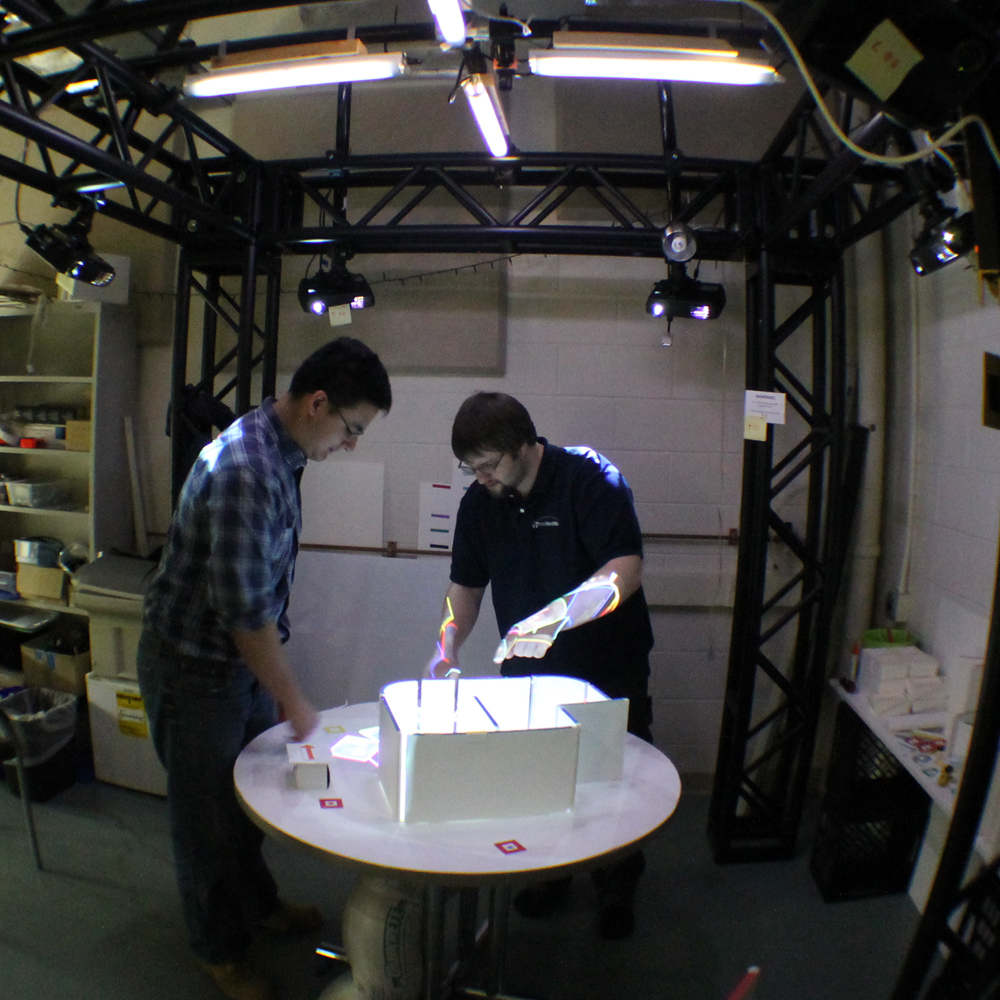
\includegraphics{images/matt_ian_fisheye}}
\resizebox{!}{3.2in}{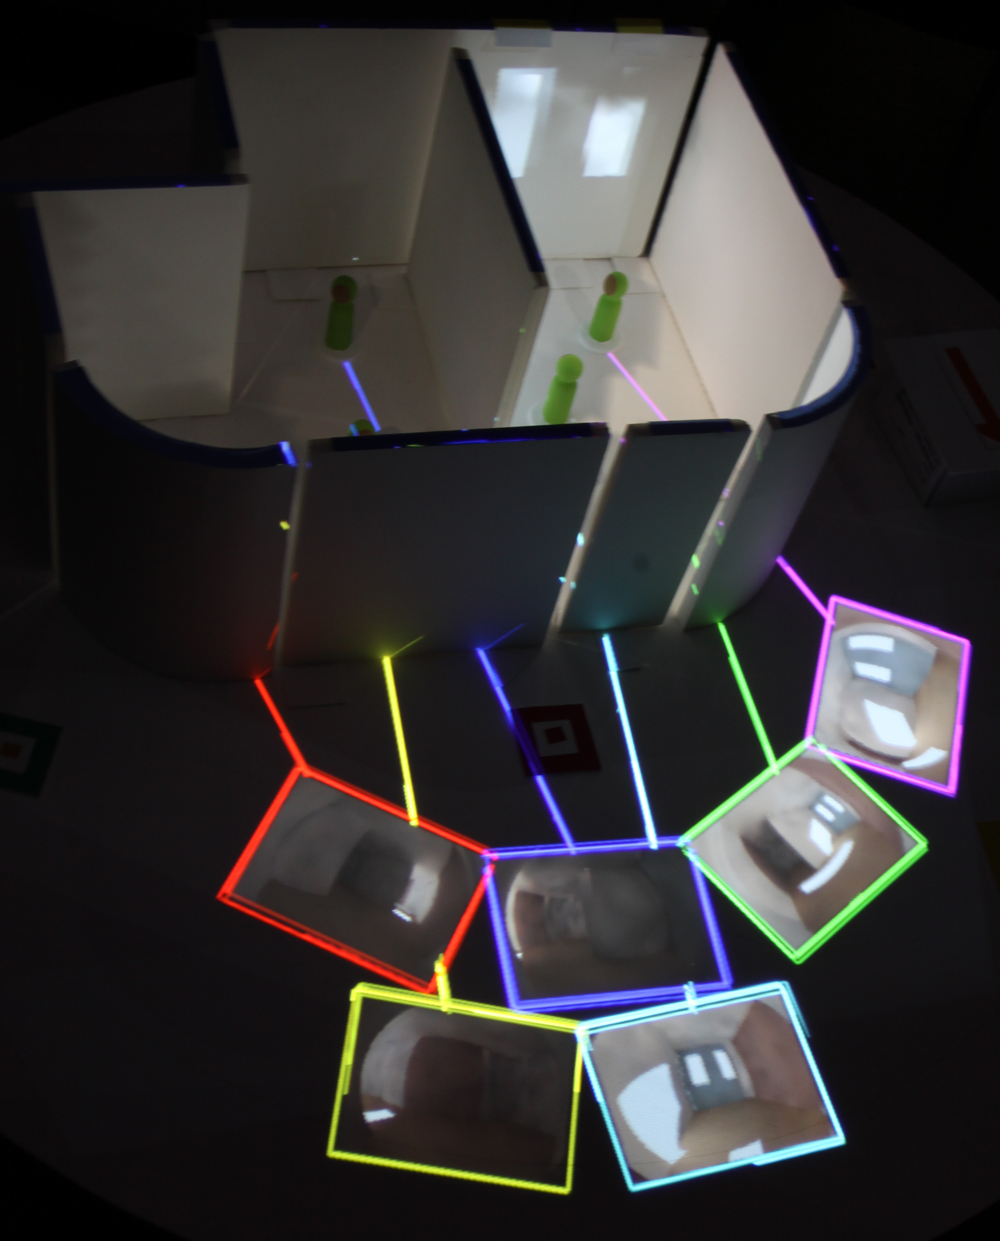
\includegraphics{images/office_color}} \\
\caption{ The Virtual Heliodon consists for 4 projectors and 1 camera
  mounted on a frame of PVC pipe with aluminum and plywood bracing.
  Users gather around a table in the center of the frame to view a
  projection of the daylighting simulation on a 3D model built of
  foamcore.}
\label{FIGURE_contraption}
\end{figure}


\begin{figure}
  \begin{center}
    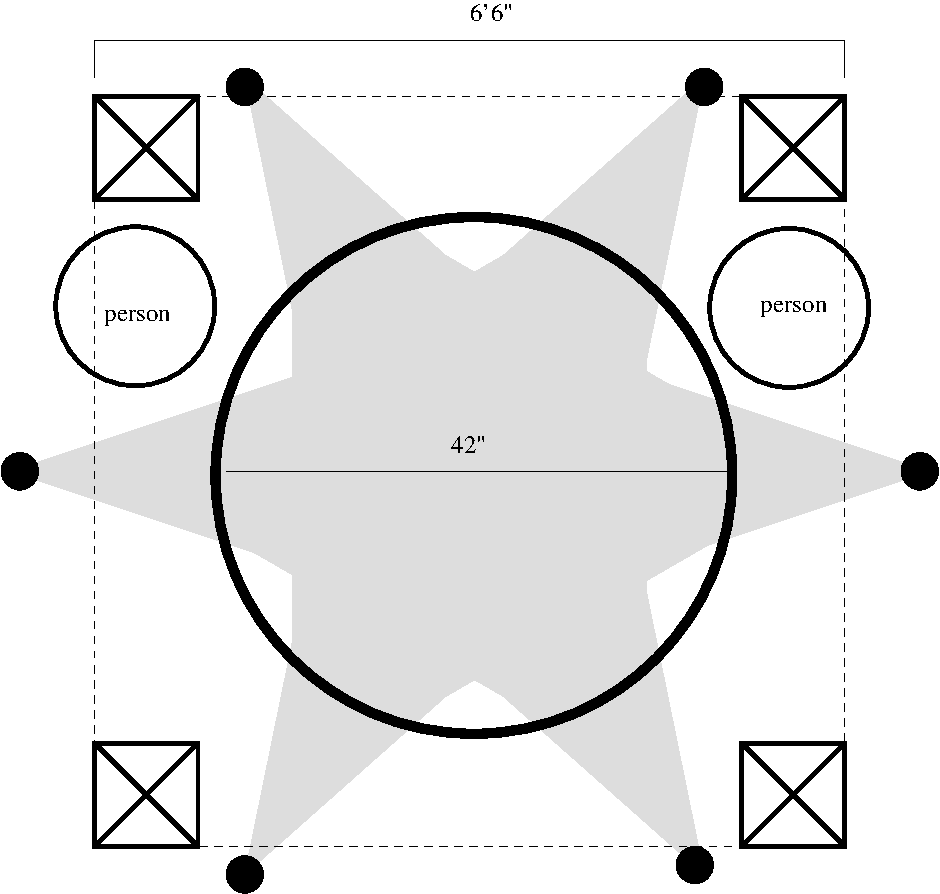
\includegraphics[width=0.45\textwidth]{images/top_view.pdf} \hfill
    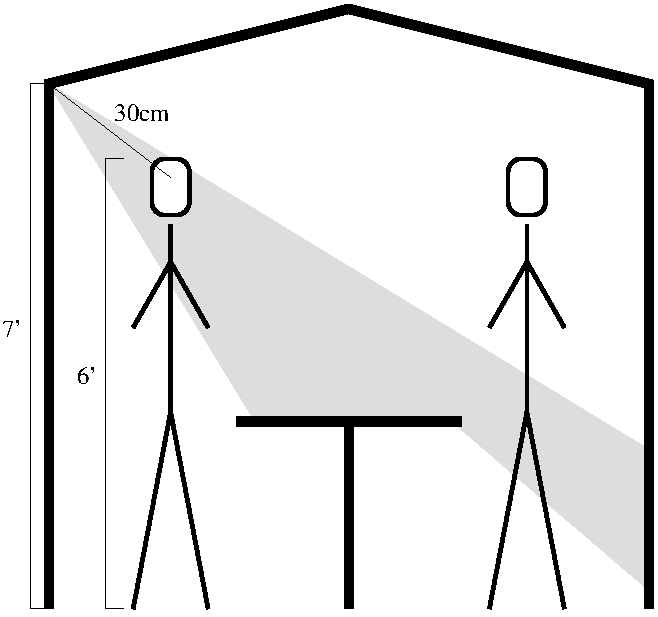
\includegraphics[width=0.5\textwidth]{images/side_view.pdf}
  \end{center}
  \caption{Diagram of system of system from the top (left) and side
    (right).  The natural place for users to stand during use of the
    system is next to the table between two uprights rather than
    between the table and one upright as this would put them in the
    beam of light and cause shadows on the table. The natural gaze of
    participants is downwards towards the table or horizontally to
    make eye contact with other users rather than directly into the
    projector lens.
\label{FIGURE_system_diagram}
}
\end{figure}






Our system (Figure~\ref{FIGURE_contraption}) centers around a standard
30'' high, 42'' diameter table.  A standard, heavy-duty stage
technology aluminum truss frame positions the camera and projectors
above the table.  The projectors and camera are securely mounted to
the frame using appropriate, commercially-available mounting brackets.
The wide stance of the frame allows more than 26'' of clearance
between each of 4 vertical uprights and the table.  Three of the four
sides of the frame are open with at least 3' of clearance.  The top
bar of the frame is 7' above the base.  

Six standard portable office projectors (each weighing approximately
7.5 lbs) are mounted in a circle above the heads of the users using a
standard mounting bracket rated to hold projectors of this size.  The distance
from the floor to the bottom of the projector is over 6'6''.  A
digital camera, weighing approximately 0.5 lbs, is positioned
approximately 8' above the floor and is secured with a standard tripod
mounting bracket.  Standard power and data cables are used to connect
the projectors, camera, and lights to three computers placed on a desk
near the frame.  The cables are neatly run along the upper bars of the
frame and attached using cable ties and the excess cable is looped and
secured next to the desk.  No cables are loose or are run along the
floor.  The system contains no custom electrical components and all
electrical components are used within their UL design specifications
and according to the manufacturer's instructions.

Standard fluorescent tube room lighting is used during operation of
the table top Spatially Augmented Reality system and will be used
throughout the duration of the study.  The average illumination in the
space is 300 lux (lumen/m$^2$).  For reference, recommended lighting
levels for normal office and laboratory work is in the range of
250-1000 lux or for precision and detailed work the recommended range
is 1500-2000 lux.  With room lighting only, the illumination on the
table surface is 300 lux.  With all 6 projectors displaying full
brightness white images, the center of the table surface is less than
20,000 lux.  For reference, noon sunlight falling on a horizontal
surface is approximately 120,000 lux.  All objects that will be placed
on the table are matte (not reflective or shiny) and thus the
brightness from the projectors and halogen lights will be uniformly
distributed in all directions and will not result in any intensely
bright specular reflections to any viewpoint.

\section{Safety of Projectors}

We are using 6 Optoma EP 727 projectors.  Each projector uses a 180W
Phillips UHP mercury lamp.  These projectors are typical small
portable projectors that are used for everyday presentations.  We have
not made any physical modifications to the case of the projector, thus
all manufacturer safety features to protect users in the event of a
bulb failure or breakage are still in place.  Similarly, we have not
made any modifications to the intensity of light output from the
projector or removed or changed any of the filters and lenses
installed in front of the bulb.  Thus, intuitively, because it is safe
to observe (for extended periods of time) the screen upon which the
image is projected, logically it is also safe to observe the table and
wall surfaces upon which these projectors display images.  We further
analyze this safety in the following section.

It is not recommended to stand in the beam of projection and look
directly at the projector.  Use of our system and our specific user
studies will never require or ask the users to gaze toward the
projector lens (Figure \ref{FIGURE_system_diagram}) and we will
caution them both verbally and through signage about the potential
eye hazard in doing so (Figure~\ref{FIGURE_warning_signs}).  However,
we note that during normal use of these and similar projectors for
class or office presentations, the presenter often does just this as
he faces the audience.  Thus, our system is well within the normal,
expected, and safe use of these devices.


\begin{figure}[t]
  \begin{center}
    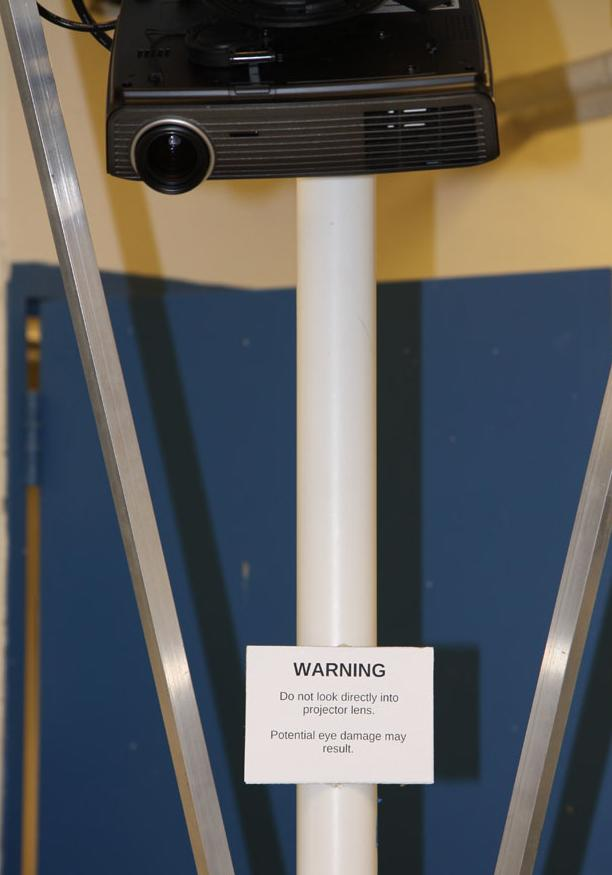
\includegraphics[width=0.3379\textwidth]{images/img_1193_small2.jpg}
    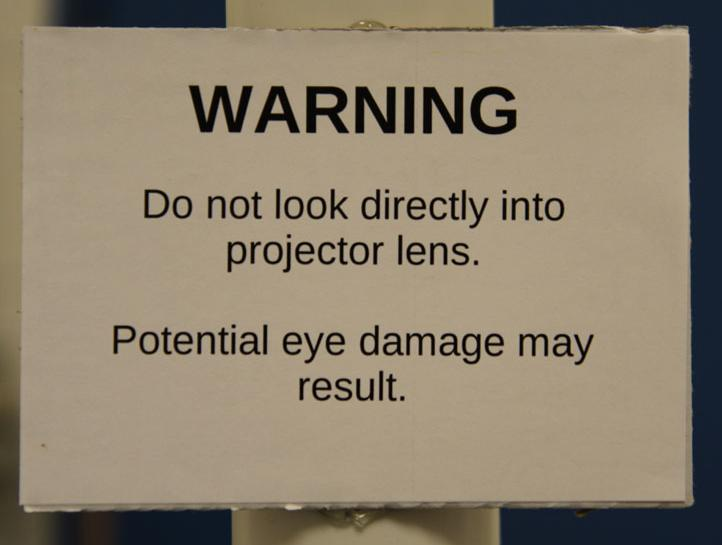
\includegraphics[width=0.64\textwidth]{images/img_1194_small2.jpg}
  \end{center}
  \caption{In addition to verbally instructing participants to avoid
    looking into the projector lens, we have installed warning signs
    near each projector at eye level, in a clearly visible position.
\label{FIGURE_warning_signs}
}
\end{figure}


We made a concerted effort to obtain safety documentation on the
intensity and spectral distribution of the light from this specific
bulb directly from the manufacturer and distributor.  We contacted
both Optoma and Phillips in December 2008 asking for the Spectral
Power Distribution (SPD) of the equipment we have purchased from
Optoma (the bulb is apparently manufactured by Phillips).  Both
companies replied within a few days and we were told that the
information was not available.  A second request to Phillips for the
same information was made on May 4th 2009.  We called 1-800-937-5483
and were told that ``UHP'' in the name of the lamp indicated that the
bulb was an OEM part, thus the data was not available.  She suggested
that we contact Optoma for the data.  She did give us the number of
the OEM division of Phillips (1-866-915-5886).  From the OEM division,
we were transferred to Technical Assistance, who spent about 30
minutes searching for the specifications, but they were ultimately
unable to locate the bulb (or any 180W projector lamp) in their
equipment catalog.
%
%They gave us the
%number of a specialty lamp division at Phillips (1-732-563-3339) and
%...
A second request to Optoma was made through their website on May 4th,
2009.  The auto-reply email said we would here from a technical
specialist within 24-48 hours, but we have not heard a response.  

Since we were not able to obtain the information directly from these
companies, we were forced to make these measurements and safety
calculations ourselves.  

%Using the SPD data and the table of the ``Spectral Weighting Functions
%for Assessing Retinal Hazards from Broad-Band Optical Sources'' the
%Blue Light Hazard Exposure Limits can be calculated [ANSI/IESNA
%  RP-27.1-05].  

%We attempted to borrow a spectroradiometer, equipment that can measure
%the SPD, to directly measure the quantity and distribution of light
%from these devices during normal operation.  Unfortunately,
%Dr. Mariana Figueiro in the RPI Lighting Research Center said her lab
%did not have equipment we could borrow.  Similarly, Dr. E. Fred
%Schubert of the Future Chips Constellation said his lab did not have
%any equipment capable of making these measurements.


\section{Blue Light Hazard Calculation Detail}

To evaluate the retinal photochemical hazard posed to study
participants by light emitted by the six projectors used in the
system, we calculated permissible time limits for exposure during an
eight-hour period in accordance with ANSI/IESNA RP-27.1-05,
specifically section 4.3.2, ``Retinal Blue Light Hazard Exposure
Limit.''  Two calculations were performed: exposure limits for the
system as it is intended to be used (study participants looking at
matte white surfaces illuminated by up to six projectors), and
accidental direct viewing of the lens of one projector from within the
beam of that projector.

During the intended use of the system, study participants will view
matte-surface card-stock and foam-core board illuminated by up to six
projectors.  For purposes of hazard evaluation, we assume 100\%
reflectivity (measured at 95\%) and Lambertian reflectance
characteristics.  We assume all six projectors are illuminating the
table in a direct-incidence configuration, which is a worst-case
situation, although not physically possible with the system
(projectors are rigidly mounted in opposing directions).  Moreover, we
assume that all six projectors produce the same spectral irradiance
at the table surface, and take this irradiance to be the maximum
measured over all six projectors (output varies due to bulb
manufacturing tolerances and degradation over bulb lifetime).

\begin{figure}[t]
  \begin{center}
    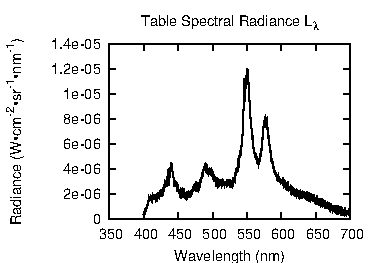
\includegraphics[width=0.6\textwidth]{images/table_radiance.pdf}
  \end{center}
  \caption{Measured worst-case radiance from table surfaces.
\label{FIGURE_worst_case_radiance}
}
\end{figure}

We measured the relative spectral output of the projectors with an
Ocean Optics spectroradiometer and calibrated the measurements at the
table surface to spectral irradiance ($W/m^2\cdot nm$) using a
calibrated luxmeter with accurate CIE $V_m(\lambda)$ characteristics
(Figure~\ref{FIGURE_worst_case_radiance}).  We evaluated the
blue-light hazard function according to the following equation
\cite{ANSI}:


\[L_B = \sum_{300}^{700}L_{\lambda}\cdot B(\lambda)\cdot \Delta \lambda\]

Given the worst-case assumptions presented above, we calculated a
blue-light hazard weighted radiance reflected from the table of
$1.73\times10^{-4}$ $W/cm^{-2}\cdot sr^{-1}$.  This value is less than
2\% of the maximum allowed for time exceeding $10^4$ seconds (2.77h)
\cite{ANSI}, a period substantially longer than the maximum 1.5 hour
study participants will be allowed to use the system.  We conclude
that there is no retinal photochemical injury hazard from the intended
use of the system.

Due to the design of the system, it is possible for study participants
to accidentally look directly into the projector.  To evaluate this
hazard, measurements were taken of the spectral radiance of the
projectors at a distance of 30cm from the projector lens, which is the
closest the eyes of a 6'-tall individual can get (measurements
obtained with projectors off). At this distance the blue light hazard
weighted radiance is $L_B = $ 43.2 $W/cm^{-2}\cdot sr^{-1}$. According
to the formula \cite{ANSI}:

\[t(max) = \frac{100}{L_B},\]

\noindent
the maximum permissible exposure is 2.3 seconds.  Since the perceived
brightness of the projectors at this distance is comparable to that of
direct noon sunlight, it is doubtful that study participants would
accidentally stare directly into the projectors for extended periods
of time, since we expect that this would be uncomfortable, and the
natural reaction would be to look away and step out of the projector
beam.  To mitigate the risk presented by possible exposure several
steps will be taken.  First, study participants will be instructed
both verbally and in writing not to look directly into the projectors
since this may cause eye damage.  Additionally, warning signs have
been posted (Figure~\ref{FIGURE_warning_signs}) in a clearly visible
location near each projector warning participants of possible eye
damage and instructing them not to look directly into the projector
lenses.  Finally, during the study the person running the study will
carefully monitor the participant and if the participant's gaze is
drawn away from the table for an extended period, they will be
encouraged to step completely away from the SAR frame to prevent
accidentally gazing into the projector lens.

As a verification of our measurement and calibration procedures, we
ran identical calculations for noon sunlight and obtained maximum
per-day exposure limits within 10\% of published results
\cite{Okuno08}.








\begin{thebibliography}{widest entry}
  \bibitem{Okuno08} Okuno, Tsutomu, ``Hazards of Solar Blue Light,'' Applied Optics, V. 47,
    No 16. June 1, 2008.
  \bibitem{ANSI} ANSI/IES RP-27.1-05, ``Photobiological Safety for Lamps and Lamp Systems -
 General Requirements,'', Illuminating Engineering Society, 2005.
\bibitem{dolce}
Dolce, Andrew, 
``Multi-User Interactions for Spatially Augmented Reality Games''
Masters Thesis, Rensselaer Polytechnic Institute, 
Department of Computer Science,
June 2011.
\url{http://www.cs.rpi.edu/graphics/theses/andrew_dolce_MS_May2011.pdf}
\end{thebibliography}



\newpage

\pagestyle{empty}

\vspace*{-0.6in}
\begin{center}
{\Large 
Institutional Review Board \\
Rensselaer Polytechnic Institute} \\
\ \\
\vspace{-0.05in}
{\large Informed Consent Form}
\end{center}
\vspace{-0.05in}
%\vspace{0.1in}

\noindent
I understand that Barbara Cutler, who is a professor of Computer
Science at Rensselaer Polytechnic Institute, wishes to interview me as
part of the research project on a new Spatially Augmented Reality (SAR)
system for education and entertainment applied to games.  I understand
that she will be making her best possible effort to guarantee me every
possible protection, including the following:

\begin{enumerate}


\vspace{-0.04in}
\item I am under no obligation to be participate in the study or to be
  interviewed if I do not wish to do so.  

\vspace{-0.04in}
\item I am not obligated to perform any of the game play exercises or
  answer any of the questions.  I may decline to answer any or all of
  the questions, and I may terminate the study or interview at
  any point, without giving any reason.

\vspace{-0.04in}
\item 
Participants for this study will be compensated for their time in the
form of a gift certificate at the rate of \$10 per hour.  This
compensation is not contingent upon the subject completing the entire
study and will be prorated if the subject withdraws.

\vspace{-0.04in}
\item I will be identified by a randomly assigned ID number that is
  used only for this study.  All recordings and game state files will be
  labeled with this ID.  All information and data relating to the user
  study will be protected to secure confidentiality.  All electronic
  files will be stored on password protected computers.  All paper
  forms will be stored in a locked office.  The correspondence
  between the ID number and my name will be recorded by Barbara Cutler
  and be accessible only by her.  This correspondence will be
  destroyed once analysis of the data is complete, within 1 year after
  participation in the study.

\vspace{-0.04in}
\item If there is anything that I do not wish to have quoted, or any
  game state files that I do not want made public, I may say at any point
  during or after the interview what I wish to have kept off the
  record and it will not be quoted or used in a publication.

\vspace{-0.04in}
\item I understand that if Barbara Cutler decides to use any portions
  of this interview or any examples of my game play in subsequent
  publications, that she will send me a copy of the portions of the
  interview and any game play, including any quotations and paraphrases
  that she decides to use, for my editing and written approval.  I
  will have the right to edit the material and I will receive a copy
  of the final publication.  She will only use the material that I
  have approved and the use of all material will be anonymous.
  I may also change my mind at any point up to and
  including the review of any quotations and paraphrases and game play
  that might be used.
\vspace{-0.05in}

\item Based on reading this form (check one): 
\vspace{-0.02in}

\noindent
\hspace*{0.3in} \rule{0.3in}{1pt} I agree to be interviewed. \\
\hspace*{0.3in} \rule{0.3in}{1pt} I do not agree to be interviewed.

\vspace{-0.04in}
\item The basic camera-projection Spatially Augmented Reality (SAR)
  setup has been described to me and I have been warned not to look
  directly at the projector lenses.  Standing close to the projector
  (30cm) and looking directly into the projector bulb for 2 seconds or
  longer may cause permanent eye damage.

\end{enumerate}

\vspace{0.3in}

\noindent
\rule{2.6in}{1pt}~~~~\rule{2.6in}{1pt}\hfill \rule{1in}{1pt}\\
\hspace*{0.7in}Name of Participant 
\hfill Signature \hspace{1.3in} 
Date \hspace{0.3in}

\vspace{0.15in}
\noindent
For further information contact:

%\vspace{0.05in}
\noindent
Barbara Cutler, Department of Computer Science, MRC 330B, cutler@cs.rpi.edu,\\
110 8th Street, Troy NY 12180; phone: (518) 276 3274, fax: (518) 276 2529.

%\vspace{0.05in}
\noindent
Institutional Review Board, Rensselaer Polytechnic Institute, CII 7015, \\
110 8th Street, Troy, New York, 12180; phone: (518) 276-4873, fax: (518) 276-4002.
\vspace{-0.8in}

\newpage

\noindent
{\bf {\Large Sample Design Exercise Instructions}}

\vspace{0.1in}

\noindent
This design exercise is based on the WoZoCo apartment complex in the
Netherlands by MVRDV (Figure~\ref{FIGURE_outside}), which consists of
100 units in (primarily) a traditional {\em single-loaded corridor}
arrangement.  The main advantage of this arrangement is that all units
have sufficient access to southern exposure and thus plenty of
daylight.  However, zoning restrictions required that 13 of the units
be relocated to the north side of the building.  This unusual
suspended arrangement required an innovative use of structural
trusses, which was justified by the increased access to daylighting
the design provided.

\begin{figure}[h]
\centering
\resizebox{!}{1.5in}{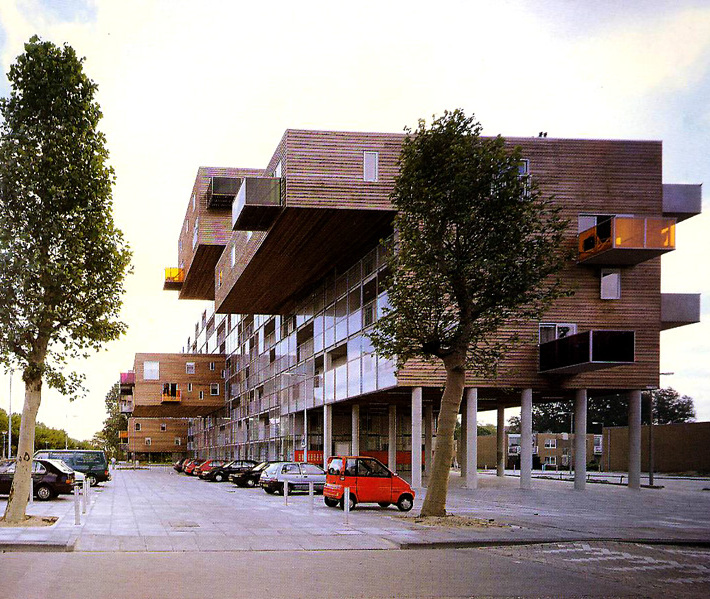
\includegraphics{wm_mvrdv10_small_crop.jpg}}
\resizebox{!}{1.5in}{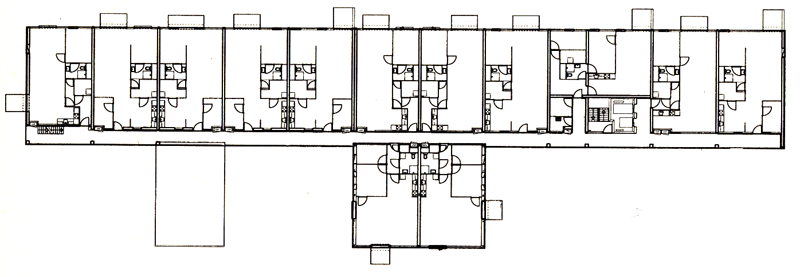
\includegraphics{plan_crop_small.png}} \\
\vspace{-0.3in}
\hspace*{4in}~$\swarrow$\\
\vspace{-0.1in}
\hspace*{4.2in}~N\\
\vspace{-0.05in}
\caption{ WoZoCo apartments, MVRDV, 1997.}
\label{FIGURE_outside}
\end{figure}



\begin{enumerate}

\item ($\sim$20 minutes) Using the physical walls, create a rough
  model that represents apartment unit on the fifth (top) floor of the
  complex and position the ``north'' arrow so that the exterior facade
  faces roughly south.  Access to the sun and sky hemisphere from the
  southern facade is unblocked by trees or neighboring buildings.
  Design the southern facade of this unit, maximizing the use of
  natural illumination within the interior, but minimizing the risk of
  overheating in the summer.  Consider the performance throughout the
  year.  You may use a variety of windows, balconies, awnings, and
  materials to give personality to this unit.  Optionally use Ecotect
  and/or LightSolve (our new software) to analyze your design.

\item ($\sim$20 minutes) Using the provided glare tokens evaluate glare in
  the space and re-design based on your findings.  The space should be able to be 
  at least 75\% utilized during the working day.  

\item ($\sim$20 minutes) Now adjust the window materials using the provided tokens.
  You may continue to use the glare tokens as well to facilitate the best daylighting possible.

\end{enumerate}


\newpage

\noindent
{\bf {\Large Sample Post-Design Questionnaire}}

\vspace{0.1in}

\begin{enumerate}

\item
What aspects of daylighting were easier to visualize and analyze with
the Virtual Heliodon, our new physical daylighting design environment?

\item
What aspects of daylighting remain easier to visualize and analyze
with the traditional software (Ecotect, etc.) or with a traditional
heliodon?

\item
Were you able to gather this information more easily or more quickly
with the Virtual Heliodon than with other tools?  Did the ease and/or
speed of access to this information improve the design process and
your final design?  Describe.

\item
Did you find the glare tokens useful in helping you evaluate the space?
If yes, in what ways did you use them to help you evaluate?

\item
Did the provided alternate window materials allow you to make signficantly different
design decisions?  If so, please describe.

\item
Sketch some designs that you were not able to evaluate due to time or
system limitations, and describe what you would like to learn about
daylighting in that space.

\item
What additional features would you like to see added to the system?

\end{enumerate}


\end{document}
